\documentclass[a4paper]{article}

%% Language and font encodings
\usepackage[english]{babel}
\usepackage[utf8x]{inputenc}
\usepackage[T1]{fontenc}
\usepackage{natbib}

%% Sets page size and margins
\usepackage[a4paper,margin=2cm]{geometry}

%% Useful packages
\usepackage{amsmath}
\usepackage{graphicx}
\usepackage[colorinlistoftodos]{todonotes}
\usepackage[colorlinks=true, allcolors=blue]{hyperref}

% This will make it easier for markers
% to refer to specific lines of your report.
\usepackage{lineno}
\linenumbers 

\title{Report title (tell us what you learned!)}
% Your report should be anonymous: it should not
% contain your name(s) or student id(s).
\date{}

\begin{document}
\maketitle

\begin{abstract}
Your abstract should briefly explain the motivation, method, analysis, and results. It needn't be more than
a few sentences.
\end{abstract}

\section{A few tips}

Use the figure environment and the caption command to add a number and a caption to your figure. See the code for Figure \ref{fig:frog} in this section for an example.

\begin{figure}
\centering
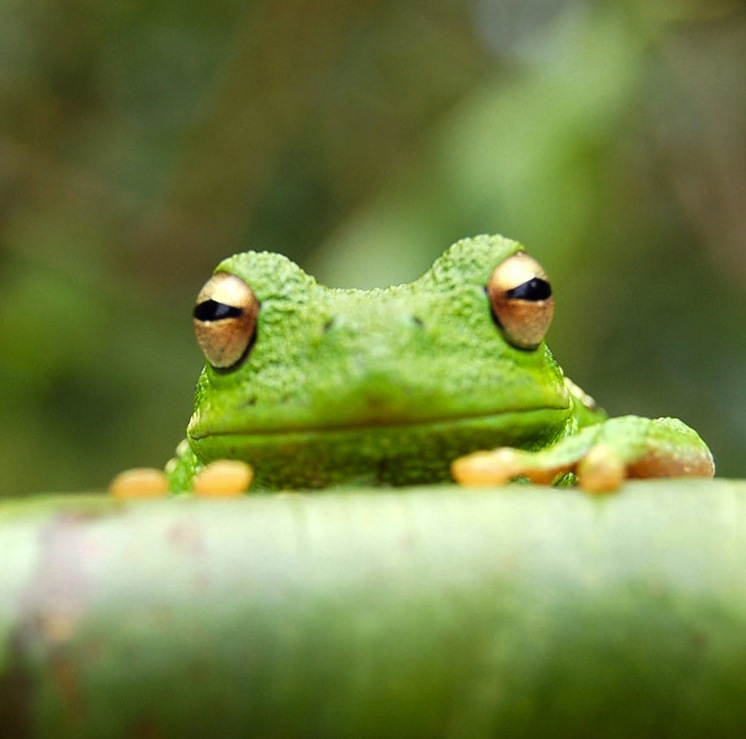
\includegraphics[width=0.3\textwidth]{frog.jpg}
\caption{\label{fig:frog}This frog was uploaded via the project menu.}
\end{figure}

\subsection{How to add Tables}

Use the table and tabular commands for basic tables --- see Table~\ref{tab:widgets}, for example. 

\begin{table}
\centering
\begin{tabular}{lr}\hline\hline
Item & Quantity \\\hline
Widgets & 42 \\
Gadgets & 13
\end{tabular}
\caption{\label{tab:widgets}An example table.}
\end{table}

\subsection{How to write Mathematics}

\LaTeX{} is great at typesetting mathematics. Let $X_1, X_2, \ldots, X_n$ be a sequence of independent and identically distributed random variables with $\text{E}[X_i] = \mu$ and $\text{Var}[X_i] = \sigma^2 < \infty$, and let
\[S_n = \frac{X_1 + X_2 + \cdots + X_n}{n}
      = \frac{1}{n}\sum_{i}^{n} X_i\]
denote their mean. Then as $n$ approaches infinity, the random variables $\sqrt{n}(S_n - \mu)$ converge in distribution to a normal $\mathcal{N}(0, \sigma^2)$.


\subsection{How to create Sections and Subsections}

Use section and subsections to organize your document. The sections and subsections create an outline of your report, and a reader should be able to infer the structure of your report just by skimming them.

\subsection{Citations and references}

We encourage you to cite research papers in your report, and to support this, you are allowed an unlimited number of pages for citations. (Aside: if a paper was posted on arxiv.org and later published in a conference or journal, please cite the published version).
There are a couple of common ways to use citations: parenthetically in running text \citep{greenwade93}; or as nouns, e.g. ``as \citet{greenwade93} showed''. Just remember to specify a bibliography style, as well as the filename of the \verb|.bib|.

\bibliographystyle{plainnat}
\bibliography{sample}

\section*{Appendix}

You may use an unlimited number of appendix pages to
include plots, tables, figures, and long examples. Equations should appear in the main text, not the Appendix. Abuse of the appendix (e.g. by including text or by putting critical information into captions when it should be in the main text) may result in loss of marks.

\end{document}